\chapter{実装}
\label{chap:implementation}

\section{実装概要}

第\ref{chap:design}章でも述べた通り、本研究では「インスリンペンを使用してインスリンが摂取された時間」と「患者本人が食事を開始した時間」を取得するため、それぞれのデバイスが必要である。
本章では、それぞれの実装内容について触れる。

\section{インスリン摂取検知デバイス}
\label{section:insulin_pen_device}

本研究におけるインスリン摂取検知デバイスは、患者のインスリン摂取を検知すると、その検知した時間をWebサーバーに対してPOSTリエストし、WebサーバーがMySQLに保存するという流れを取っている。
図\ref{fig:insulin_injection_flow}にこの実装部分の概略と、フローを示す。

\begin{figure}[htbp]
  \caption{インスリン摂取検知デバイスの概略とフロー}
  \label{fig:insulin_injection_flow}
  \begin{center}
    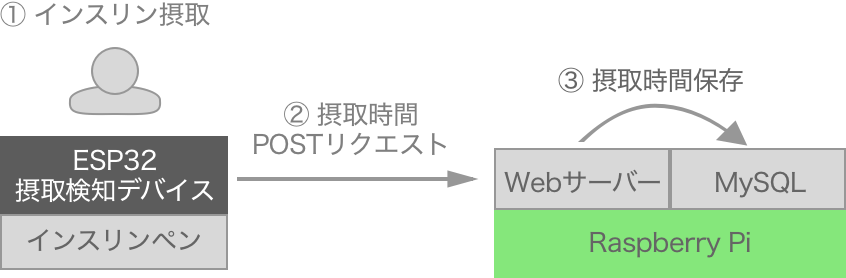
\includegraphics[bb=0 0 1000 270,width=18cm]{assets/insulin_injection_flow.png}
  \end{center}
\end{figure}

\subsection{環境}

インスリン摂取を検知するためのインスリンペンデバイスは以下の機器で構成される。

\begin{table}[htbp]
  \caption{インスリンデバイスの実装環境}
  \label{tb:insulin-device}
  \begin{center}
    \begin{tabular}{|c||c|}
      \hline
      開発言語  & C++ \\\hline
      通信機器  & ESP32 devkit v1(図\ref{fig:esp32}) \\\hline
      注射器を模したもの & ネームペン (図\ref{fig:insulin_pen})\\\hline
    \end{tabular}
  \end{center}
\end{table}

\begin{figure}[htbp]
  \caption{今回使用したESP32 devkit v1}
  \label{fig:esp32}
  \begin{center}
    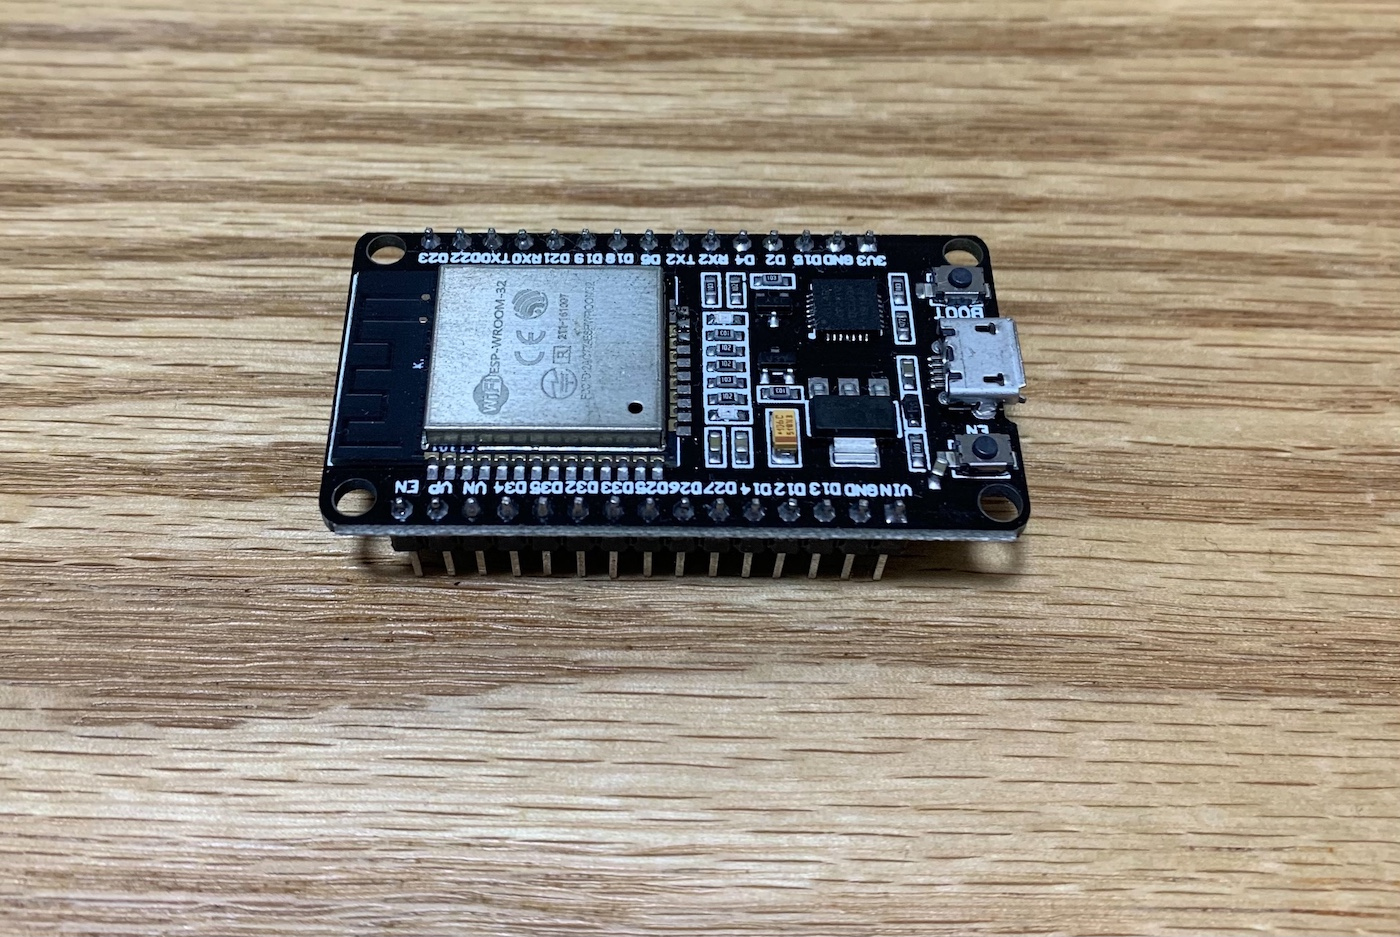
\includegraphics[bb=0 0 1300 1100,width=10cm]{assets/esp32.jpg}
  \end{center}
\end{figure}

\begin{figure}[htbp]
  \caption{今回使用したインスリン注射器の代用のためのペン}
  \label{fig:insulin_pen}
  \begin{center}
    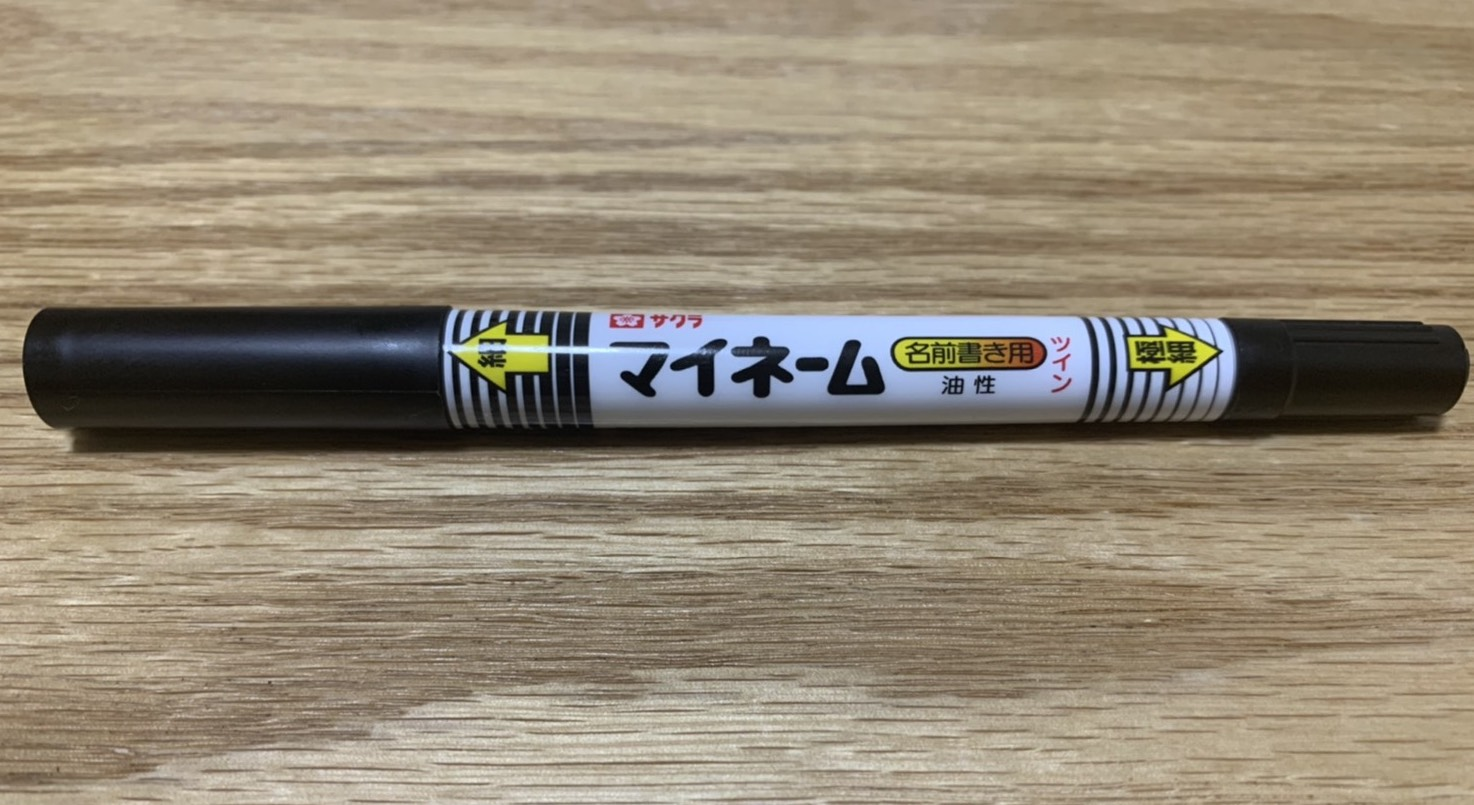
\includegraphics[bb=0 0 1400 900,width=10cm]{assets/pen.jpg}
  \end{center}
\end{figure}


アップロード先のWebサーバーは、食事検知に使用するRaspberry Pi上にホストした。
使用した言語、フレームワークは表\ref{tb:web_server}の通りである。

\begin{table}[htbp]
  \caption{Webサーバーのスペック}
  \label{tb:web_server}
  \begin{center}
    \begin{tabular}{|c||c|}
      \hline
      開発言語  & Python 3.7.3 \\\hline
      フレームワーク  & Flask 1.0.2 \\\hline
      DB & MySQL ver 15.1 Distrib 10.3.25-MariaDB \\\hline
    \end{tabular}
  \end{center}
\end{table}

\subsection{実装内容}

インスリン注射器の端のボタンが一定時間以上押された場合に摂取と判定する構造を作るため、今回は物理的なタクタイルスイッチを接着し、このボタンが押された場合にのみ、
インスリンが摂取されたとして判定するよう実装した。

配線は図\ref{fig:esp32_switch}に示した。実際には、この配線を半田付けした小さい基板をネームペンの端に取り付けてインスリン検知デバイスとして扱う。
ESP32の3.3vの出力を利用し、タクタイルスイッチを通してpin34に繋ぎ、プルダウン抵抗は220Ωとした。
そしてこのスイッチが押されることで通電し、pin34でその電流を読み取る実装である。

\begin{figure}[htbp]
  \caption{ESP32とタクタイルスイッチの配線図}
  \label{fig:esp32_switch}
  \begin{center}
    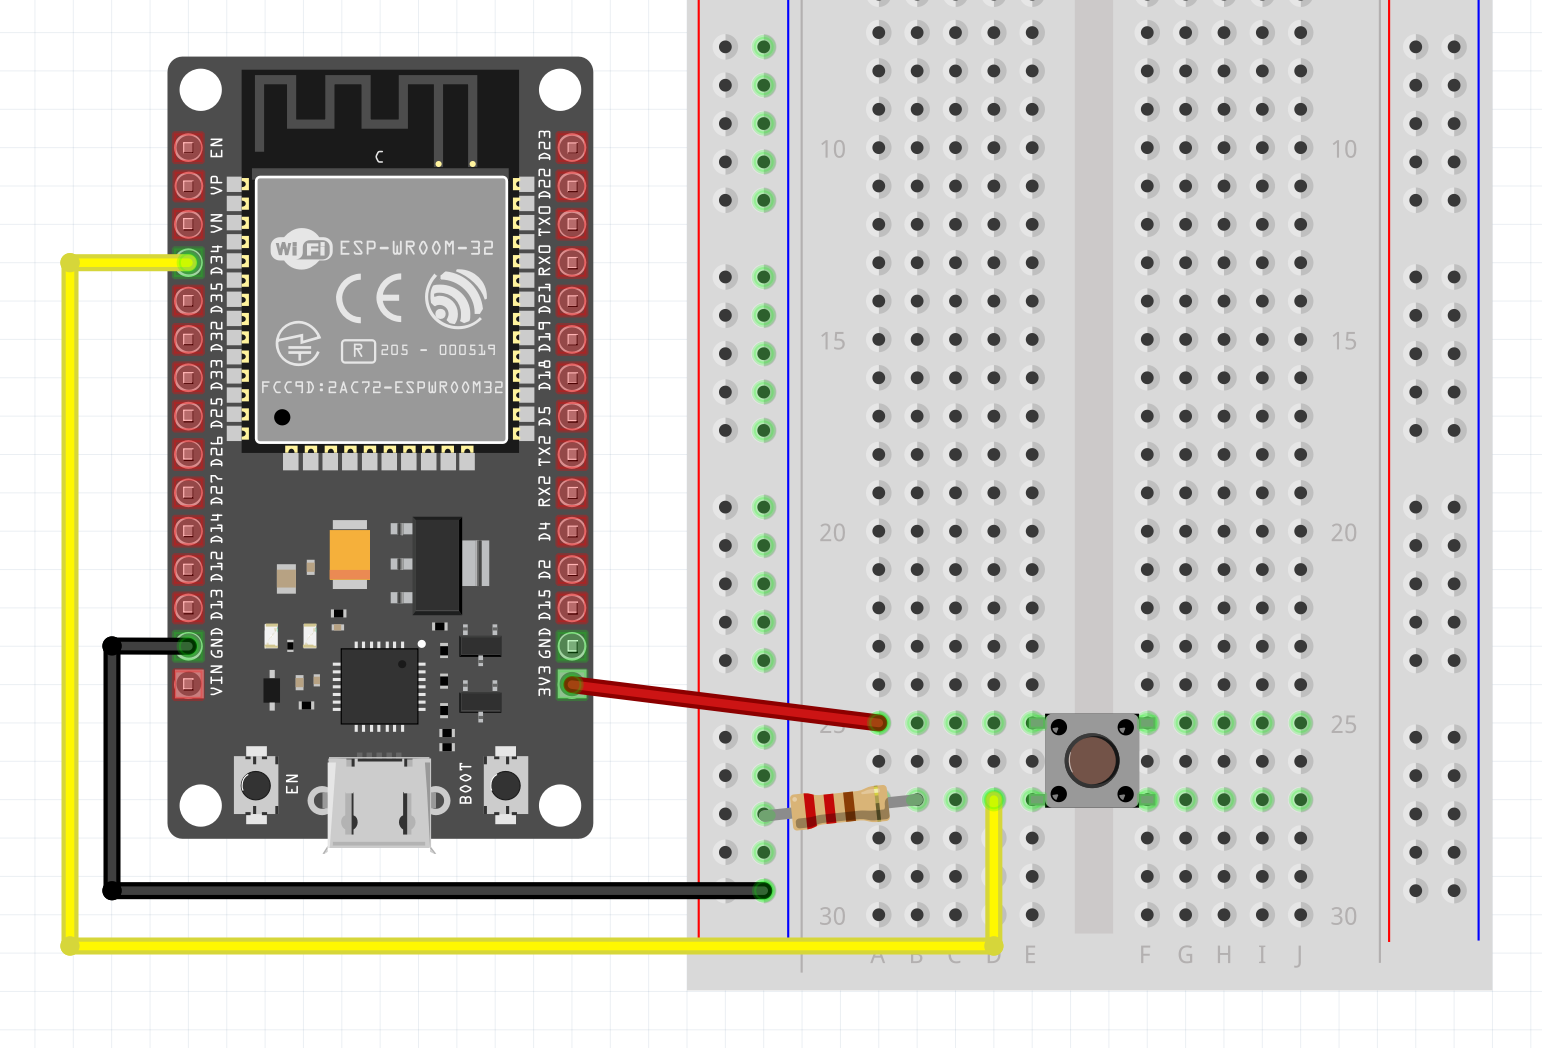
\includegraphics[bb=0 0 1000 550,width=17cm]{assets/esp32_switch.png}
  \end{center}
\end{figure}

図\ref{fig:pen_with_switch_n_esp32}が実際の実装物である。
形状や携帯性に関する配慮を行った設計や実装は本研究の本質ではないため、今回の実装内容としては省いた。

\begin{figure}[htbp]
  \caption{擬似インスリン注射器として用意したペンに今回の実装物を装着した様子}
  \label{fig:pen_with_switch_n_esp32}
  \begin{center}
    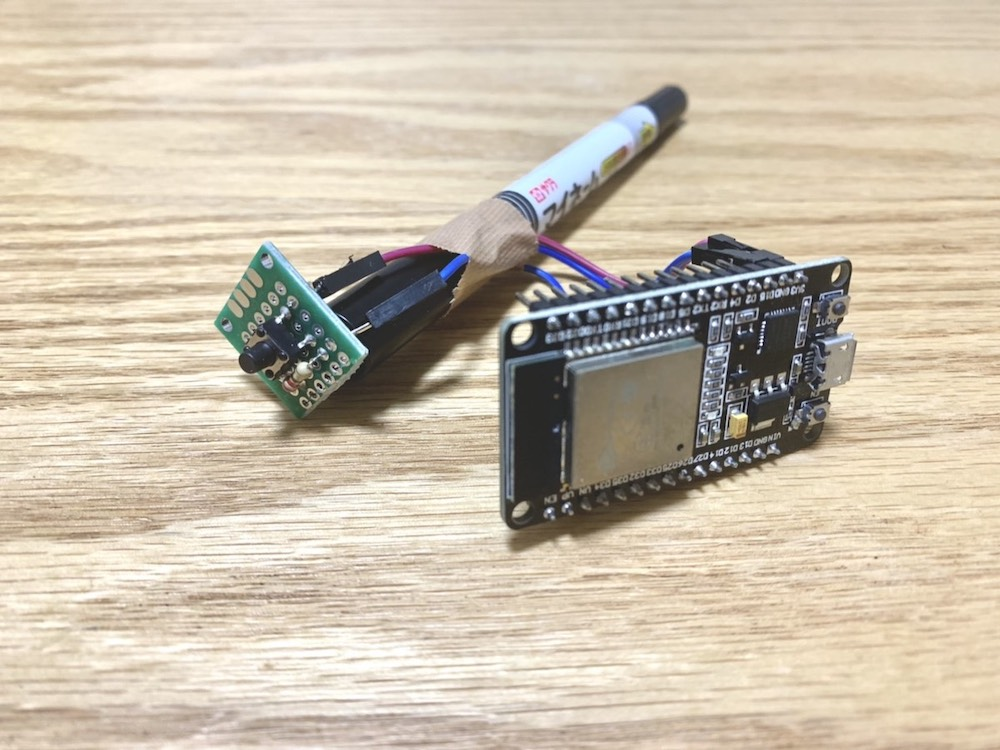
\includegraphics[bb=0 0 1050 740,width=15cm]{assets/pen_with_switch_n_esp32.jpg}
  \end{center}
\end{figure}

図\ref{fig:insulin_injection_test}が実装したインスリンデバイスを使った時の電流の変化である。
横軸を時刻、縦軸をデジタル読み取りの0,1で取った。
ここにある通り、指によってインスリンペンの端が押下されると、一時的に電流が流れ、ESP32のpin34で電流が読み取れていることがわかる。
今回は、検知と判定するための押下時間の閾値は5秒以上とした。\cite{how_to_inject_insulin_1} \cite{how_to_inject_insulin_2}

\begin{figure}[htbp]
  \caption{インスリン検知デバイスを使った時のデジタル読み取りのデータ}
  \label{fig:insulin_injection_test}
  \begin{center}
    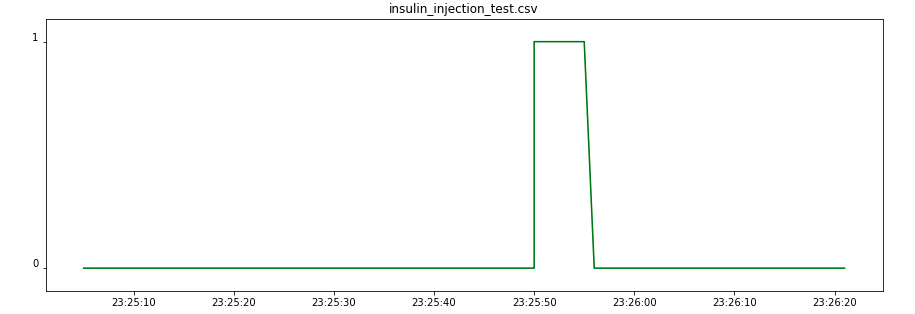
\includegraphics[bb=0 0 1000 350,width=17cm]{assets/insulin_injection_test.png}
  \end{center}
\end{figure}

本インスリンデバイスは、インスリン摂取を検知すると、HTTPプロトコルのPOSTメソッドを使用して、検知時間をJSONデータとしてWebサーバーにリクエストを行う。
POSTリクエストを受け取ったサーバーは、受け取ったデータをデコードし、摂取時間のタイムスタンプを取得、MySQLに保存する。
今回使用したPOSTリクエストのBodyのデータフォーマットは以下である。
タイムスタンプにはUnix time stampを採用した。

\begin{verbatim}
  {
    "injected_time": "1610081373"
  }
\end{verbatim}

\section{食事検知、通知}

今回、食事の検知は食卓上に鎮座させる加速度センサーによる手法を採用した。食事検知スクリプトは、食事を検知すると、
Webサーバーを経由して保存されたインスリン摂取時間を確認し、その時間と、食事時間の差異を確認した後、閾値よりも大きかった場合に患者にインスリン摂取忘れを通知する。
図\ref{fig:meal_detector_flow}に実装部分の概略とフローを示した。

\begin{figure}[htbp]
  \caption{食事検知の概略とフロー}
  \label{fig:insulin_injection_flow}
  \begin{center}
    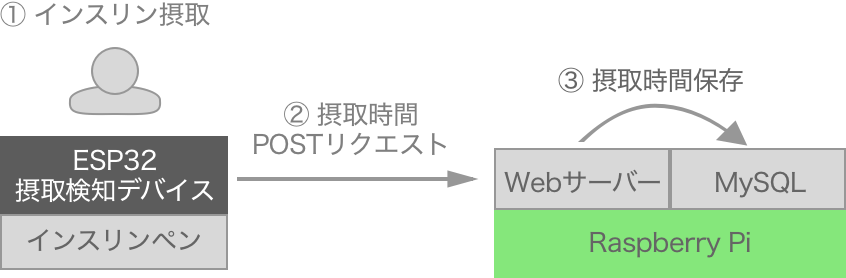
\includegraphics[bb=0 0 1000 270,width=18cm]{assets/insulin_injection_flow.png}
  \end{center}
\end{figure}

\subsection{環境}

\begin{table}[htbp]
  \caption{食事検知に使用したセンサー及びPC}
  \label{tb:meal_detection_spec}
  \begin{center}
    \begin{tabular}{|c||c|}
      \hline
      加速度センサー & ADXL345 \\\hline
      PC & Raspberry Pi 4 Model B (SD: 32GB) \\\hline
    \end{tabular}
  \end{center}
\end{table}

\begin{table}[htbp]
  \caption{ソフトウェア関連環境}
  \label{tb:meal_detection_spec_sw}
  \begin{center}
    \begin{tabular}{|c||c|}
      \hline
      開発言語 & Python 3.7.3 \\\hline
      使用ライブラリ &  time, datetime, busio, board, adafruit\_adxl34x \\\hline
    \end{tabular}
  \end{center}
\end{table}

\begin{figure}[htbp]
  \caption{加速度センサーADXL345}
  \label{fig:adxl345}
  \begin{center}
    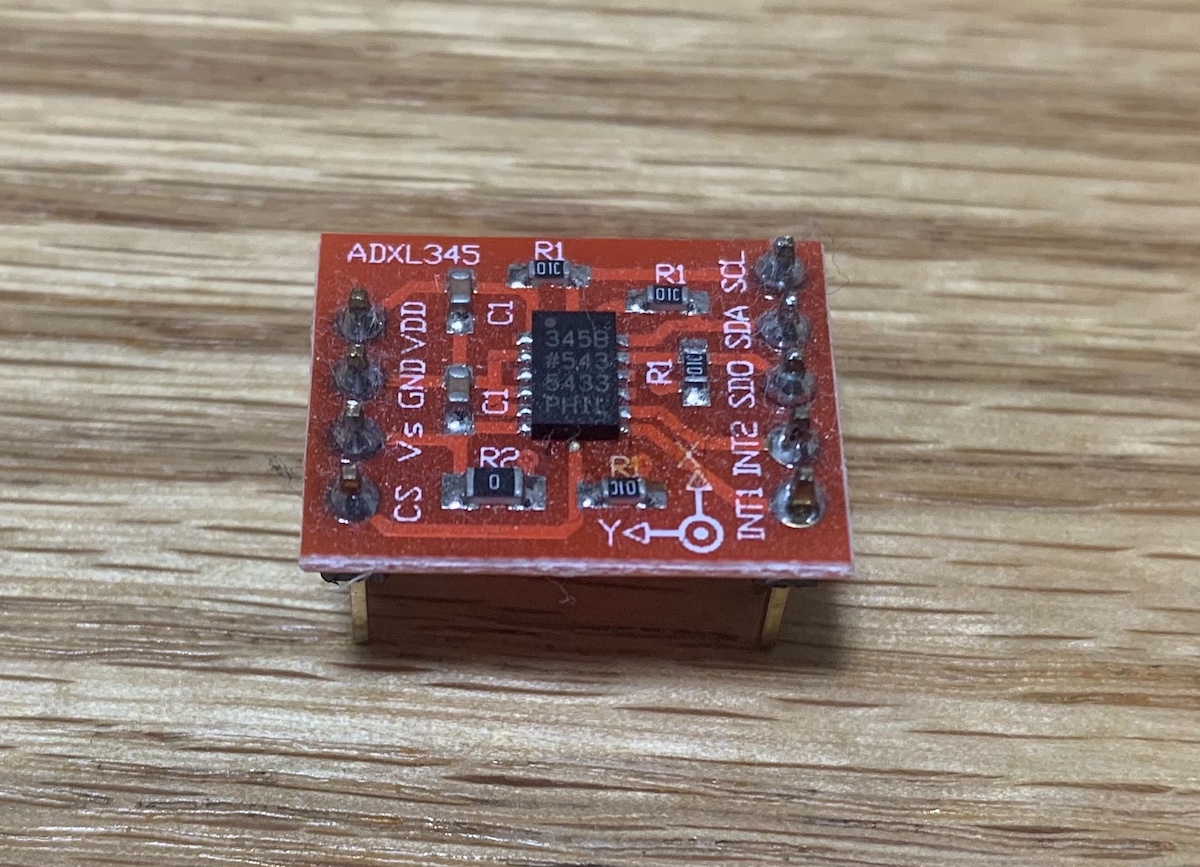
\includegraphics[bb=0 0 1300 1000,width=10cm]{assets/adxl345.jpg}
  \end{center}
\end{figure}

ADXL345は3軸加速度センサーであり、縦、横、高さの3つの値を取得することができる。今回はこの高さを使って振動を検知した。

\begin{figure}[htbp]
  \caption{Raspberry Pi 4 Model B}
  \label{fig:raspi4_model_b}
  \begin{center}
    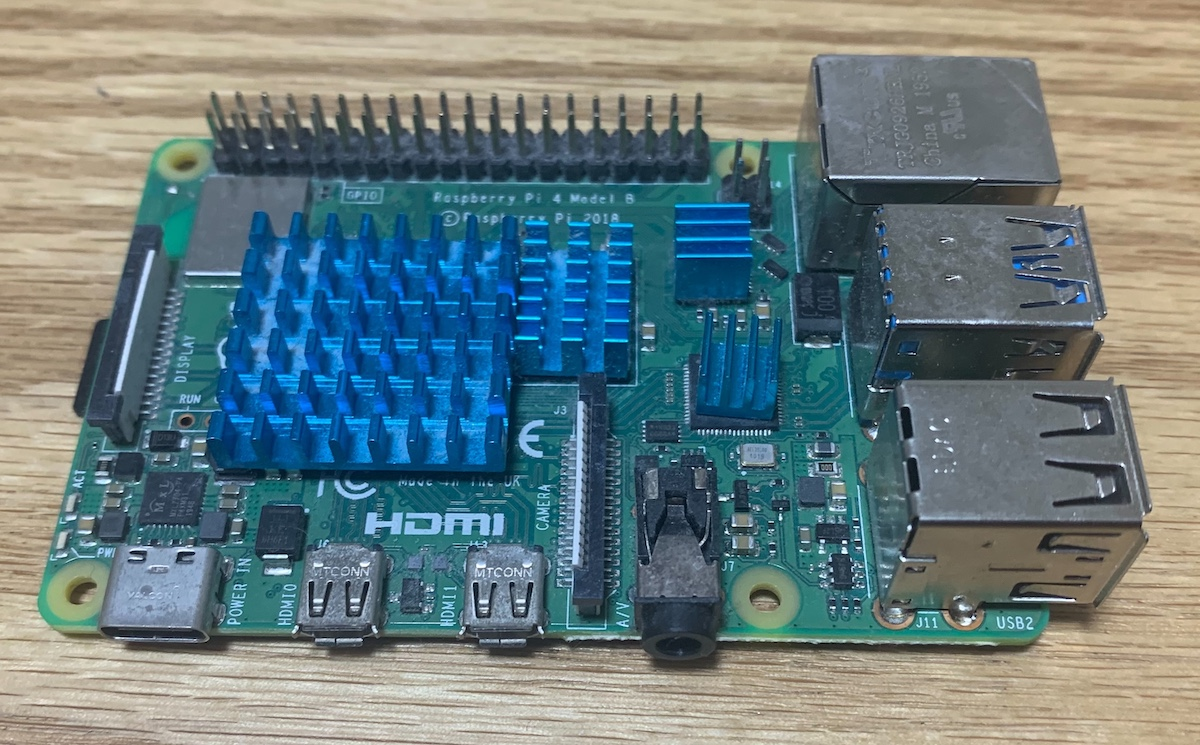
\includegraphics[bb=0 0 1300 800,width=10cm]{assets/raspi4_model_b.jpg}
  \end{center}
\end{figure}

表\ref{tb:raspberry_pi_spec}に、本研究で使用したRaspberry Piのスペックを示す。

\begin{table}[htbp]
  \caption{Raspberry Piのスペック}
  \label{tb:raspberry_pi_spec}
  \begin{center}
    \begin{tabular}{|c||c|}
      \hline
      OS  & Raspbian GNU/Linux 10 (buster) \\\hline
      CPU & Broadcom BCM2711, quad-core Cortex-A72 (ARM v8) 64-bit SoC @ 1.5GHz \\\hline
      RAM & 4GB LPDDR4-3200 SDRAM \\\hline
      Storage & Micro-SD (32GB) \\\hline
      GPIO & 40-pin GIPO header \\\hline
    \end{tabular}
  \end{center}
\end{table}

\subsection{実装内容}

今回使用したRaspberry Pi 4 Model Bは、3番ピンがSDA(Serial Data), 5番ピンがSCL(Serial Clock)に対応しており、
これらのピンを使用することにより、I2Cプロトコルを利用してセンサーデータを取得することが可能である。
通常、Raspberry PiのデフォルトではI2C通信は無効化されているため、実装前に有効化する必要がある。
そして、これら2つのピンを、加速度センサーであるADXL345の、SDAとSCLに対応するピンにそれぞれ接続し、デジタル・インタフェース電源電圧、電源電圧、そしてグラウンドを接続することで配線が完了する。\cite{adxl345_datasheet}

データを読み取り、食事を検知するスクリプトの実装には、様々なボードを使ったハードウェア開発に対応するCircuitPythonを使用した。
boardモジュールは、使用されているボードを認識し、使用可能なピンを認識し、それぞれのピンに変数名を割り当てる。これによりSDAとSCLピンを取得し、I2C通信に使用することが可能となる。
I2C通信の確立には、busioモジュールのI2Cクラスを使用し、データの取得を行うために、デバイスドライバであるadafruit\_adxl34xを使用した。
このデバイスドライバのADXL345クラスに、I2Cクラスのインスタンスと、接続されたADXL345のI2Cバスにおけるアドレスを渡すことで、ソフトウェアからセンサーデバイスの値を取得、検知可能となる。
ソースコード\ref{sensor_code}が、センサーデータ読み取りをするための簡易的な擬似コードである。

\begin{lstlisting}[caption=センサーデータを読み取るための疑似コード,label=sensor_code]
  import board
  import busio
  import adafruit_adxl34x

  i2c = busio.I2C(board.SCL, board.SDA)
  accelerometer = adafruit_adxl34x.ADXL345(i2c, address=0x1d)
\end{lstlisting}

図\ref{fig:meal_detector_wire_illustration}に配線図を示す。

\begin{figure}[htbp]
  \caption{Raspberry Pi 4とADXL345の配線図}
  \label{fig:meal_detector_wire_illustration}
  \begin{center}
    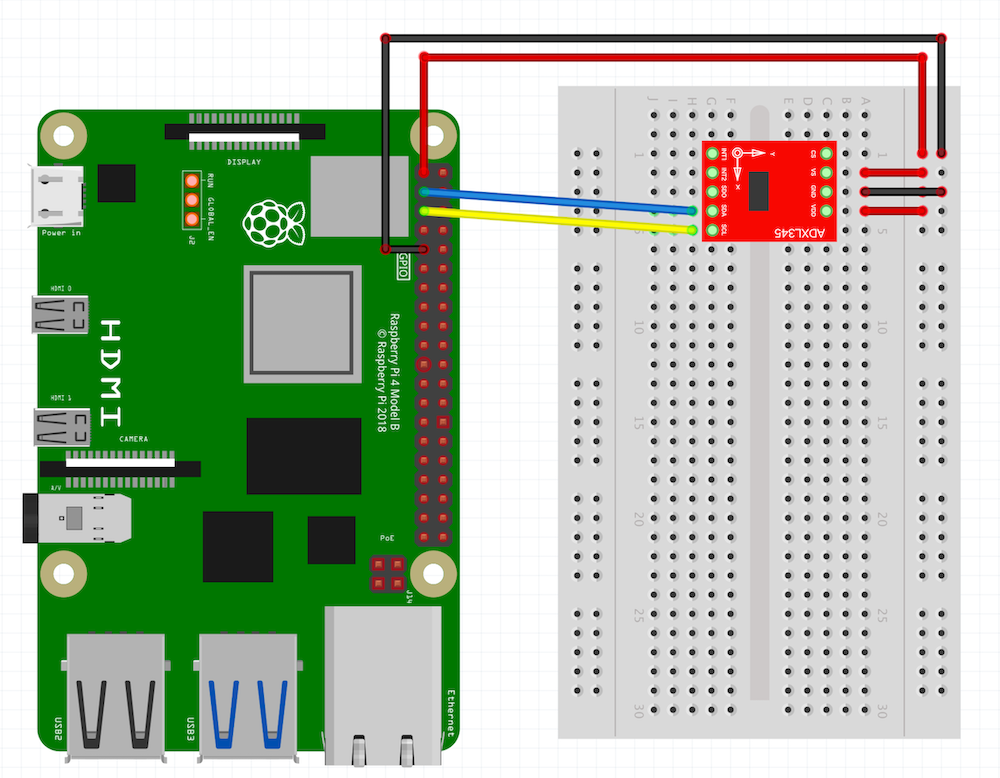
\includegraphics[bb=0 0 1000 800,width=15cm]{assets/raspi_adxl345.png}
  \end{center}
\end{figure}

そして、図\ref{fig:meal_detector}が、図\ref{fig:meal_detector_wire_illustration}に従って配線した実物である。
検知を実施する際には、これを電源に繋ぎ、動作温度を0度から50度に保つためファンを取り付けた。\cite{raspi_4_heat} \cite{raspi_4_spec}

\begin{figure}[htbp]
  \caption{配線したRaspberry Pi 4とADXL345}
  \label{fig:meal_detector}
  \begin{center}
    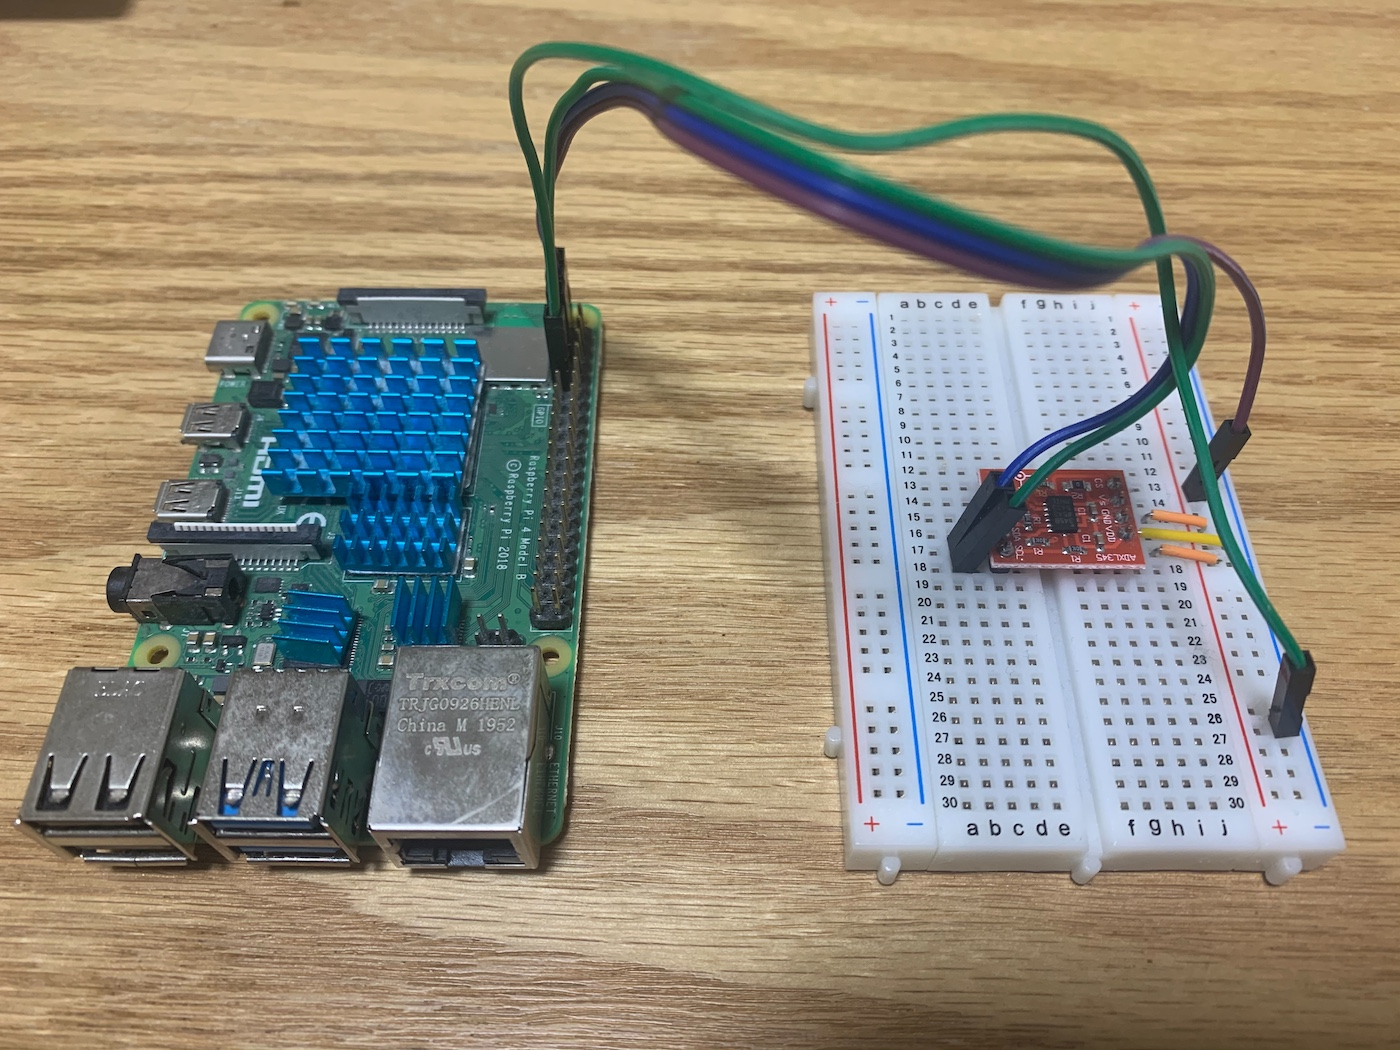
\includegraphics[bb=0 0 1300 1100,width=10cm]{assets/meal_detector.jpg}
  \end{center}
\end{figure}

\subsection{インスリン摂取忘れ通知}

上記で実装した、2つのデバイスから取得できたデータをもとにインスリンの打ち忘れ検知を行い、打ち忘れが起こった場合には、患者に対して通知を行う。
今回は、食事検知、Webサーバーのホストに使用したRaspberry Piにスピーカーを取り付け、そこから「You forgot your insulin injection」というセリフを流すことで、
患者に知らせる。図\ref{fig:system_flow}が、全体のフローであり、図\ref{fig:raspi_with_speaker}がスピーカーが取り付けられたRaspberry Piである。
スピーカーは〇〇を使用した。

インスリンの摂取から食事検知、そして患者への通知まで、一連の流れを実装モジュールと共に図\ref{fig:system_flow}にまとめた。
7の通知は、6の摂取時間を確認、比較した際に30分以上離れていた場合にのみ行われるのが今回の実装である。

\begin{figure}[htbp]
  \caption{今回実装されたインスリン摂取忘れ通知一連の流れ}
  \label{fig:system_flow}
  \begin{center}
    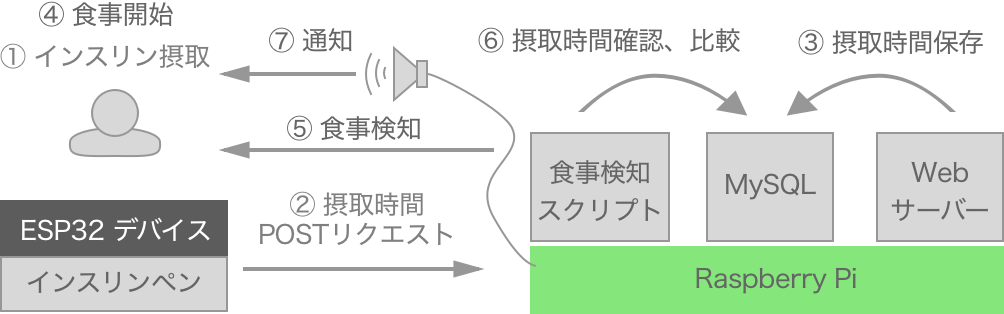
\includegraphics[bb=0 0 1000 400,width=15cm]{assets/system_flow_with_modules.png}
  \end{center}
\end{figure}

\begin{figure}[htbp]
  \caption{音声通知用にスピーカーを付けたRaspberry Pi 4}
  \label{fig:raspi_with_speaker}
  \begin{center}
    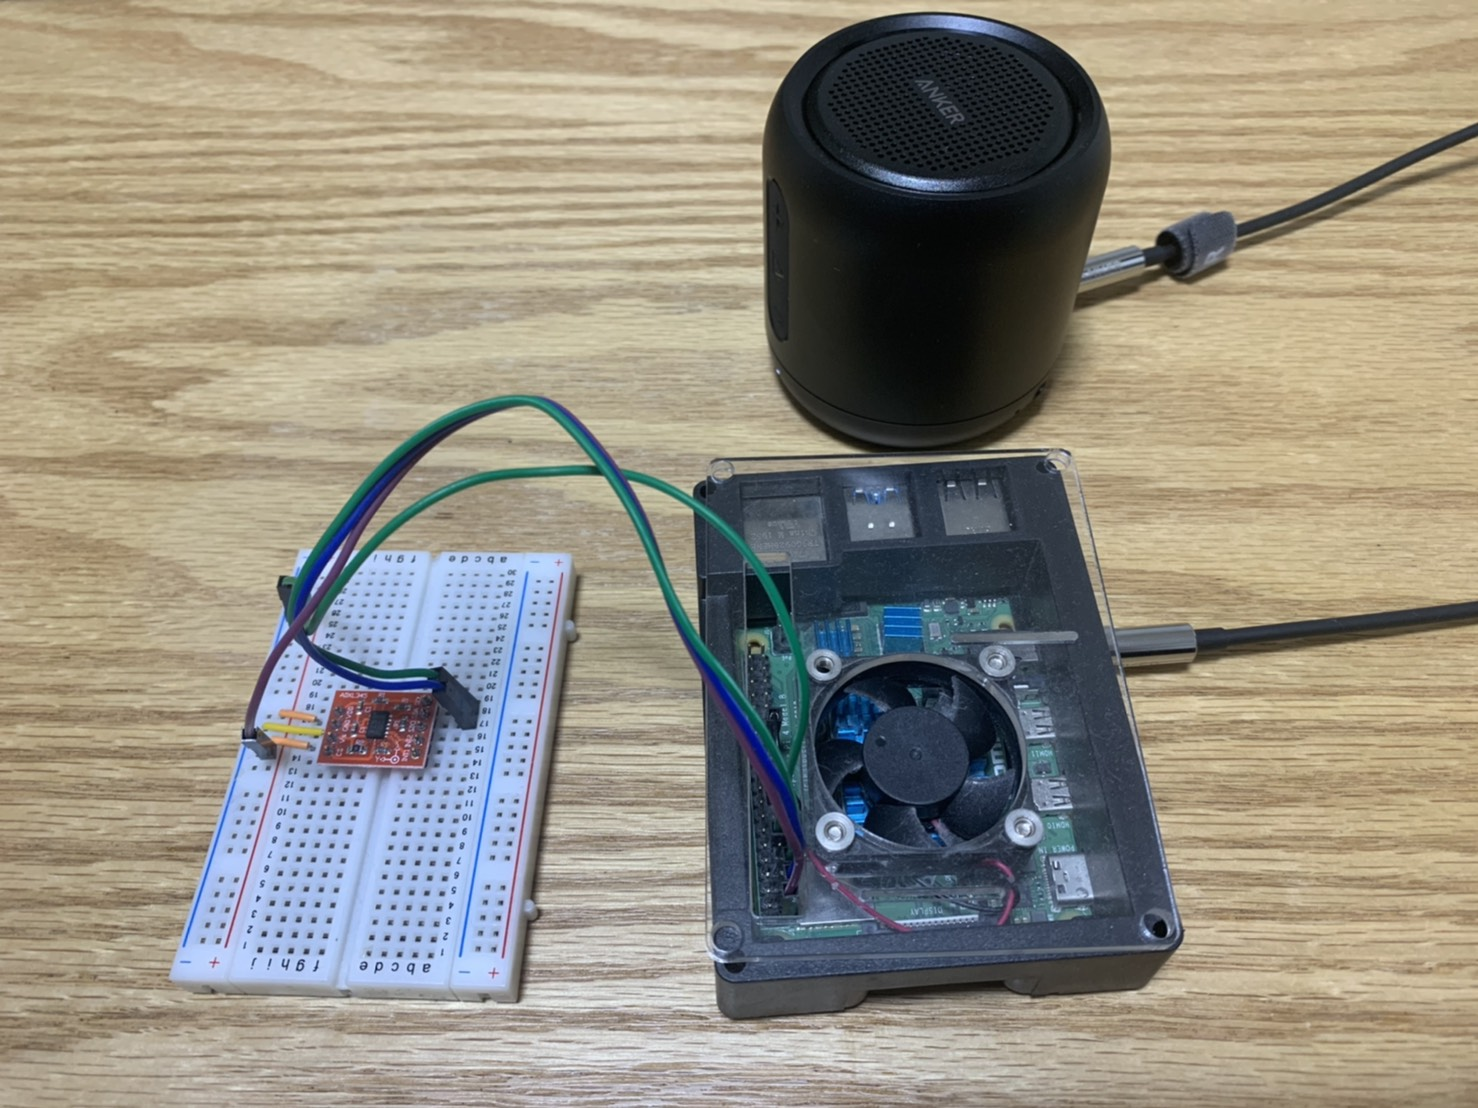
\includegraphics[bb=0 0 1400 1100,width=10cm]{assets/raspi_with_speaker.jpg}
  \end{center}
\end{figure}
